\documentclass[a4paper, 12pt]{article}%тип документа

%%%Библиотеки
	%\usepackage[warn]{mathtext}	
	\usepackage[T2A]{fontenc} % кодировка
	\usepackage[utf8]{inputenc} % кодировка исходного текста
	\usepackage[english,russian]{babel} % локализация и переносы
	\usepackage{caption}
	\usepackage{listings}
	\usepackage{amsmath,amsfonts,amssymb,amsthm,mathtools}
	\usepackage{wasysym}
	\usepackage{graphicx}%Вставка картинок правильная
	\usepackage{float}%"Плавающие" картинки
	\usepackage{wrapfig}%Обтекание фигур (таблиц, картинок и прочего)
	\usepackage{fancyhdr} %загрузим пакет
	\usepackage{lscape}
	\usepackage{xcolor}
	\usepackage[normalem]{ulem}
	\usepackage{hyperref}

%%%Конец библиотек




%%%Настройка ссылок
	\hypersetup
	{
		colorlinks=true,
		linkcolor=blue,
		filecolor=magenta,
		urlcolor=blue
	}
%%%Конец настройки ссылок


%%%Настройка колонтитулы
	\pagestyle{fancy}
	\fancyhead{}
	\fancyhead[L]{Лабораторная работа}
	\fancyhead[R]{Талашкевич Даниил, группа Б01-009}
	\fancyfoot[C]{\thepage}
%%%конец настройки колонтитулы



							\begin{document}
						%%%%Начало документа%%%%


%%%Начало титульника
\begin{titlepage}

	\newpage
	\begin{center}
		\normalsize Московский физико-технический институт \\(госудраственный 			университет)
	\end{center}

	\vspace{6em}

	\begin{center}
		\Large Лабораторная работа по электричеству\\
	\end{center}

	\vspace{1em}

	\begin{center}
		\large \textbf{Закон  [3.4.2]}
	\end{center}

	\vspace{2em}

	\begin{center}
		\large Талашкевич Даниил Александрович\\
		Группа Б01-009
	\end{center}

	\vspace{\fill}

	\begin{center}
	Долгопрудный \\2021
	\end{center}
	
\end{titlepage}
%%%Конец Титульника



%%%Настройка оглавления и нумерации страниц
	\thispagestyle{empty}
	\newpage
	\tableofcontents
	\newpage
	\setcounter{page}{1}
%%%Настройка оглавления и нумерации страниц


					%%%%%%Начало работы с текстом%%%%%%
					
\textbf{Цель работы} : изучение температурной зависимости магнитной восприимчивости ферромагнетика выше точки Кюри.

\textbf{В работе используются} : катушка самоиндукции с образцом из гадолиния, термостат, частотомер, цифровой вольтметр, $L C$-автогенератор, термопара медь-константан.
                    
\section{Теоретическое введение}


Коэффициент самоиндукции катушки $L$ пропорционален магнитной проницаемости $\mu$ заполняющей его среды (почему?): $L \propto \mu$. Тогда разность самоиндукций катушки с образцом $L$ и без него $L_{0}$ будет пропорциональна восприимчивости образца $\chi$ :
$$
L-L_{0} \propto \mu-1=\chi
$$
При изменении индуктивности образца меняется период колебаний автогенератора:
$$
\tau=2 \pi \sqrt{L C}
$$
где $C$ - ёмкость контура автогенератора. Период колебаний в отсутствие образца определяется самоиндукцией пустой катушки:
$$
\tau_{0}=2 \pi \sqrt{L_{0} C}
$$
Отсюда находим

$$
L-L_{0} \propto \tau^{2}-\tau_{0}^{2}
$$
и, следовательно,
$$
\chi \propto \tau^{2}-\tau_{0}^{2}
$$
Из формул 2 и 3 следует, что закон Кюри-Вейсса справедлив, если выполнено соотношение
$$
\frac{1}{\tau^{2}-\tau_{0}^{2}} \propto T-\Theta_{p}
$$
Измерения проводятся в интервале температур от $14^{\circ} \mathrm{C}$ до $40^{\circ} \mathrm{C}$. С целью экономии времени следует начинать измерения с низких температур.



\section{Экспериментальная установка}

В работе изучается температурная зависимость $\chi(T)$ гадолиния при температурах выше точки Кюри. Выбор материала определяется тем, что его точка Кюри лежит в диапазоне комнатных температур.

\begin{figure}[h!]
    \centering
	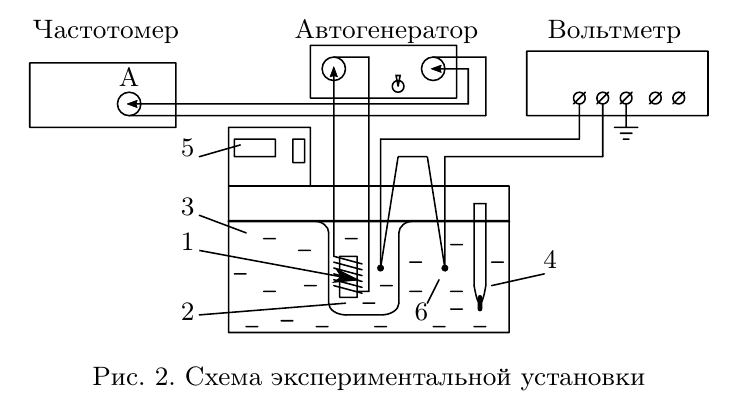
\includegraphics[width = \textwidth]{1.png}
    \caption{Схемы экспериментальных установок}
    \label{scheme}
\end{figure}

Схема установки для проверки закона Кюри-Вейсса показана на рис. 2 Исследуемый ферромагнитный образец (гадолиний) расположен внутри пустотелой катушки самоиндукции, которая служит индуктивностью колебательного контура, входящего в состав $L C$-автогенератора (генератора колебаний с самовозбуждением).

Гадолиний является хорошим проводником электрического тока, а рабочая частота генератора достаточно велика $(\sim 50$ кГц), поэтому для уменьшения вихревых токов образец изготовлен из мелких кусочков размером около 0,5 мм. Катушка 1 с образцом помещена в стеклянный сосуд 2, залитый трансформаторным маслом. Масло предохраняет образец от окисления и способствует ухудшению электрического контакта между отдельными частичками образца. Кроме того, оно улучшает тепловой контакт между образцом и термостатируемой (рабочей) жидкостью 3 в термостате. Ртутный термометр 4 используется для приближенной оценки температуры. Температура образца регулируется с помощью термостата 5 .


\section{Ход работы}


\section{Обработка результатов}


\section{Вывод}
 
\section{Литература}

\begin{enumerate}

\item \textbf{Лабораторный практикум по общей физике:} Учебное пособие. В трех томах. Т. 2. Электричество и магнетизм /Гладун А.Д., Александров Д.А., Берулёва Н.С. и др.; Под ред. А.Д. Гладуна - М.: МФТИ, 2007. - 280 с.

\end{enumerate}		
		


\end{document}